\specialsection{Language}{}{black}{white}

\subsection{The Origins}
\begin{figure}
    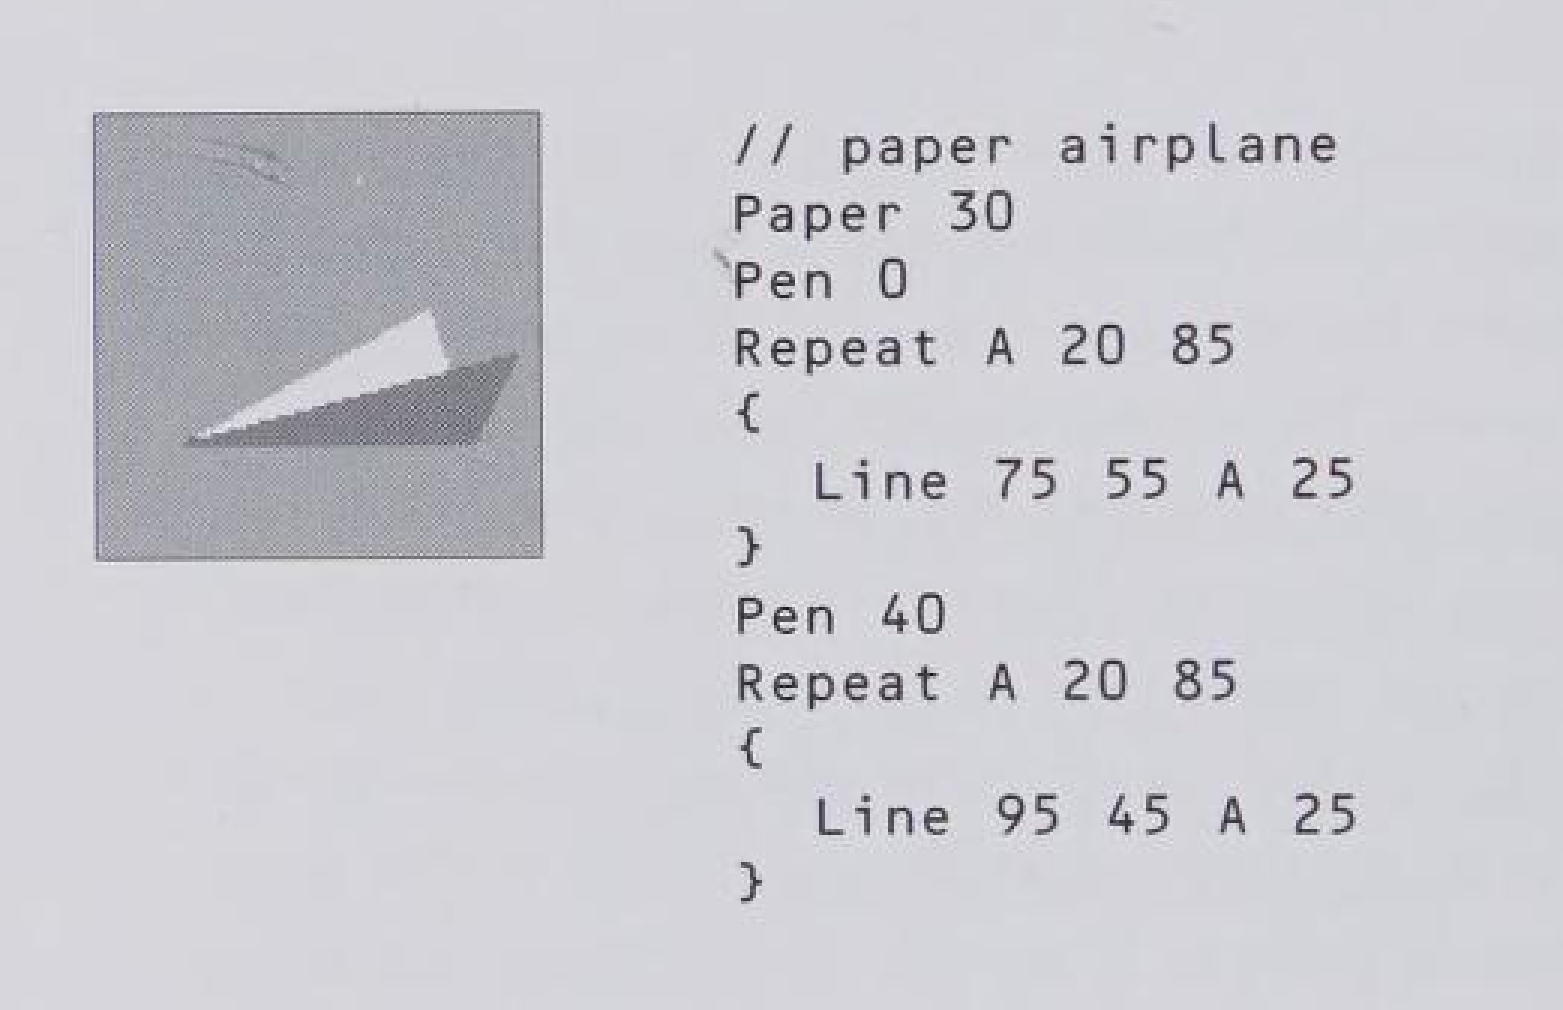
\includegraphics[max width=\textwidth]{images/dbn.png} 
    \caption{Design By Numbers Example \parencite[66]{maedaDesignNumbers2001}}
    \label{fig:dbn}
  \end{figure}

The conceptualization of Processing is intricately linked to the environment at the MIT Media Lab's Aesthetics + Computation Group (ACG). Under the leadership of John Maeda, the ACG embraced a philosophy that dismantled traditional academic divisions between technological and artistic disciplines. Maeda articulated this vision by stating, "Hybrids that can fluidly cross the chasm between technology and the arts are mutations in the academic system...During the 1990s the mutants that managed to defy this norm would either seek me out, or else I would reach out to find them myself. Bringing these unique people together was my primary passion, and that’s how I came into contact with Casey Reas and Ben Fry" \parencite{reasProcessingProgrammingHandbook2007a}.

The necessity for Processing emerged from a critical assessment of the limitations inherent in computational design tools at the time. Systems like OpenGL required extensive boilerplate code for rudimentary tasks, a process detailed in appendix \ref{lst:hello-triangle}, impeding the fluidity of visual experimentation. This challenge highlighted the need for a platform conducive to the iterative processes typical within artistic practices.

Design by Numbers (DBN)\parencite{maedaDesignNumbers2001}, an earlier project led by Maeda and tought by Reas and Fry, presented an accessible introduction to programming concepts, yet its scope was limited—operating within a monochrome color scheme and constrained to a 100x100 pixel canvas. These constraints, along with the limited command set of DBN (illustrated in figure \ref{fig:dbn}), were reminiscent of Seymour Papert's work with LOGO and its associated turtle graphics. The turtle graphics system, represented in figure \ref{fig:turtle-commands}, was similarly characterized by a limited set of commands geared towards educational purposes.

This realization of DBN's limitations was particularly pronounced during Reas and Fry's workshops with students at the Rhode Island School of Desing (RISD), where the need for a more expressive and flexible tool was evident\parencite{fryModernPrometheusHistory2018}. The response to this need was Fry's creation of Bagel, the 2D rendering engine which laid the groundwork for Processing's graphic capabilities that would offer an array of graphic primitives, such as arc(), ellipse(), line(), point(), quad(), rect(), and triangle(), and represented a significant departure from the more complex programming requirements of Java or Lingo, as delineated in table \ref{table:processing_java_comparison}.

Fry's experience with the advanced graphics framework ACU, inspirations from Flash and Director, and developing and teaching DBN culminated in the creation of Processing. This evolution was a response to the pedagogical and practical challenges faced in teaching computational design, aiming to expand beyond the black-and-white, pixel-restricted canvas of DBN to a platform that could accommodate the breadth and depth of artistic expression.

\begin{figure}
    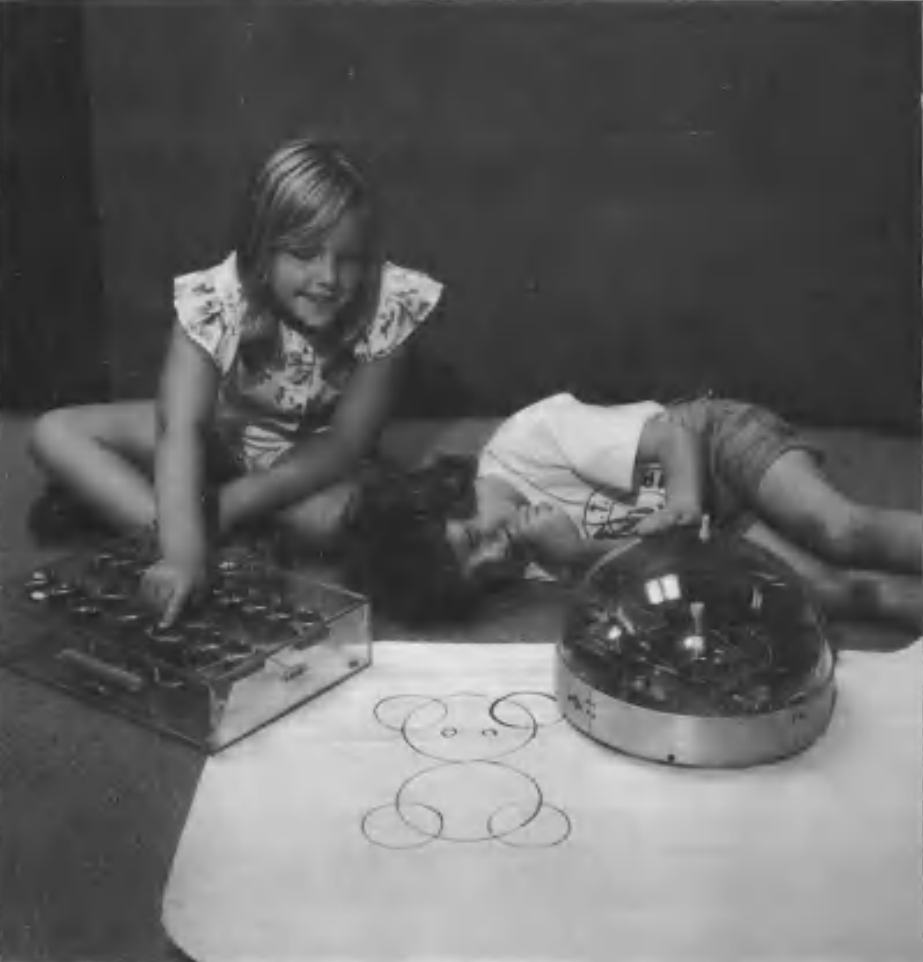
\includegraphics[max width=\textwidth]{images/turtle.png}
    \caption{Physical turtle \parencite[ii]{papertMindstormsChildrenComputers1980}}
    \label{fig:turtle-commands}
  \end{figure}

  \begin{figure}
    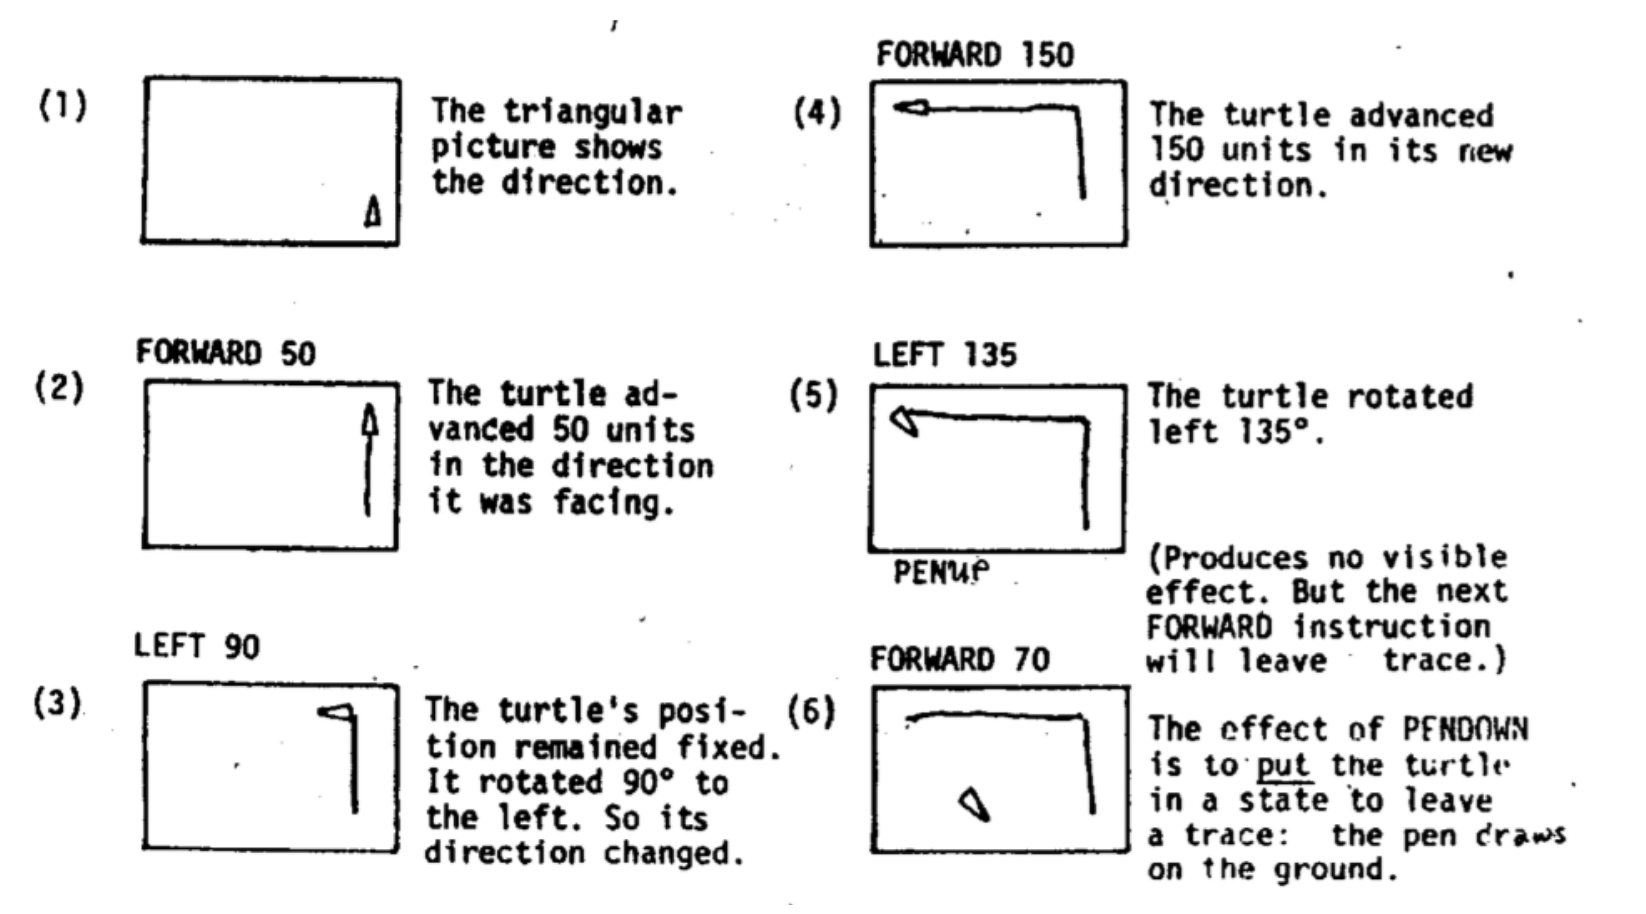
\includegraphics[max width=\textwidth]{images/turtle-commands.png} 
    \caption{Turtle Commands \parencite[827]{solomonHistoryLogo2020a}}
    \label{fig:turtle-commands}
  \end{figure}

\begin{figure}
    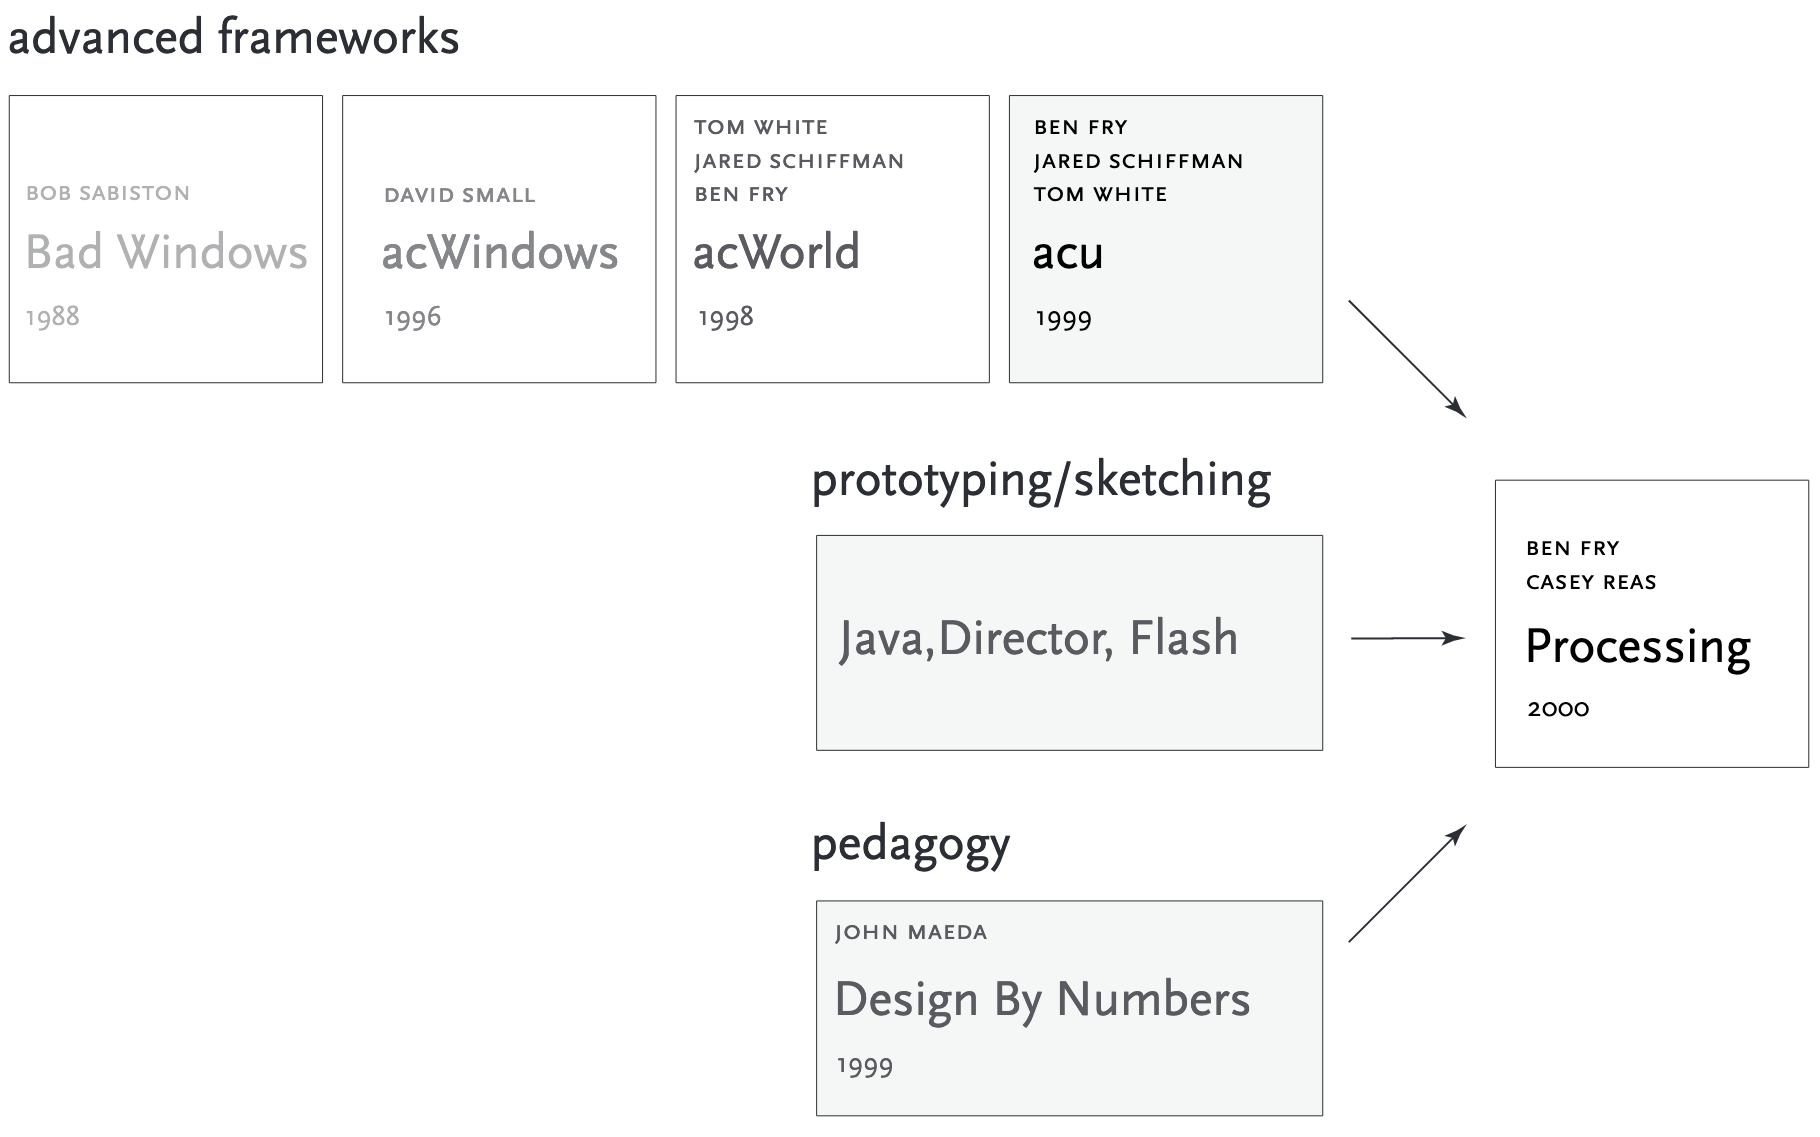
\includegraphics[max width=\textwidth]{images/fry2004-frameworks.png} 
    \caption{Precursors of Processing \parencite[127]{fryComputationalInformationDesign2004}}
    \label{fig:dbn}
  \end{figure}

\begin{table}[h!]
    \begin{adjustbox}{center}
    \begin{tabular}{|l|l|}
    \hline
    Processing & Java \\
    \hline
    \texttt{background(0);} & \makecell[l]{\texttt{g.setColor(Color.black);}\\\texttt{fillRect(0, 0, size.width, size.height);}} \\
    \hline
    \texttt{background(255);} & \makecell[l]{\texttt{g.setColor(Color.white);}\\\texttt{fillRect(0, 0, size.width, size.height);}} \\
    \hline
    \texttt{background(255, 204, 0);} & \makecell[l]{\texttt{g.setColor(new Color(255, 204, 0));}\\\texttt{fillRect(0, 0, size.width, size.height);}} \\
    \hline
    \texttt{stroke(255);} & \makecell[l]{\texttt{g.setColor(Color.white)}} \\
    \hline
    \texttt{stroke(0);} & \makecell[l]{\texttt{g.setColor(Color.black)}} \\
    \hline
    \texttt{stroke(255, 204, 0);} & \makecell[l]{\texttt{g.setColor(new Color(255, 204, 0));}} \\
    \hline
    \texttt{fill(0, 102, 153);} & \makecell[l]{\texttt{g.setColor(new Color(0, 102, 153));}} \\
    \hline
    \texttt{point(30, 20);} & \makecell[l]{\texttt{g.drawLine(30, 20, 30, 20);}} \\
    \hline
    \texttt{line(0, 20, 80, 20);} & \makecell[l]{\texttt{g.drawLine(0, 20, 80, 20);}} \\
    \hline
    \texttt{rect(10, 20, 30, 30);} & \makecell[l]{\texttt{g.fillRect(10, 20, 30, 30);}\\\texttt{g.drawRect(10, 20, 30, 30);}} \\
    \hline
    \end{tabular}
    \end{adjustbox}
    \caption{Comparison of Processing and Java library commands for graphics.}
    \label{table:processing_java_comparison}
    \end{table}

  \newpage 

  \begin{figure}[h]
    \centering
    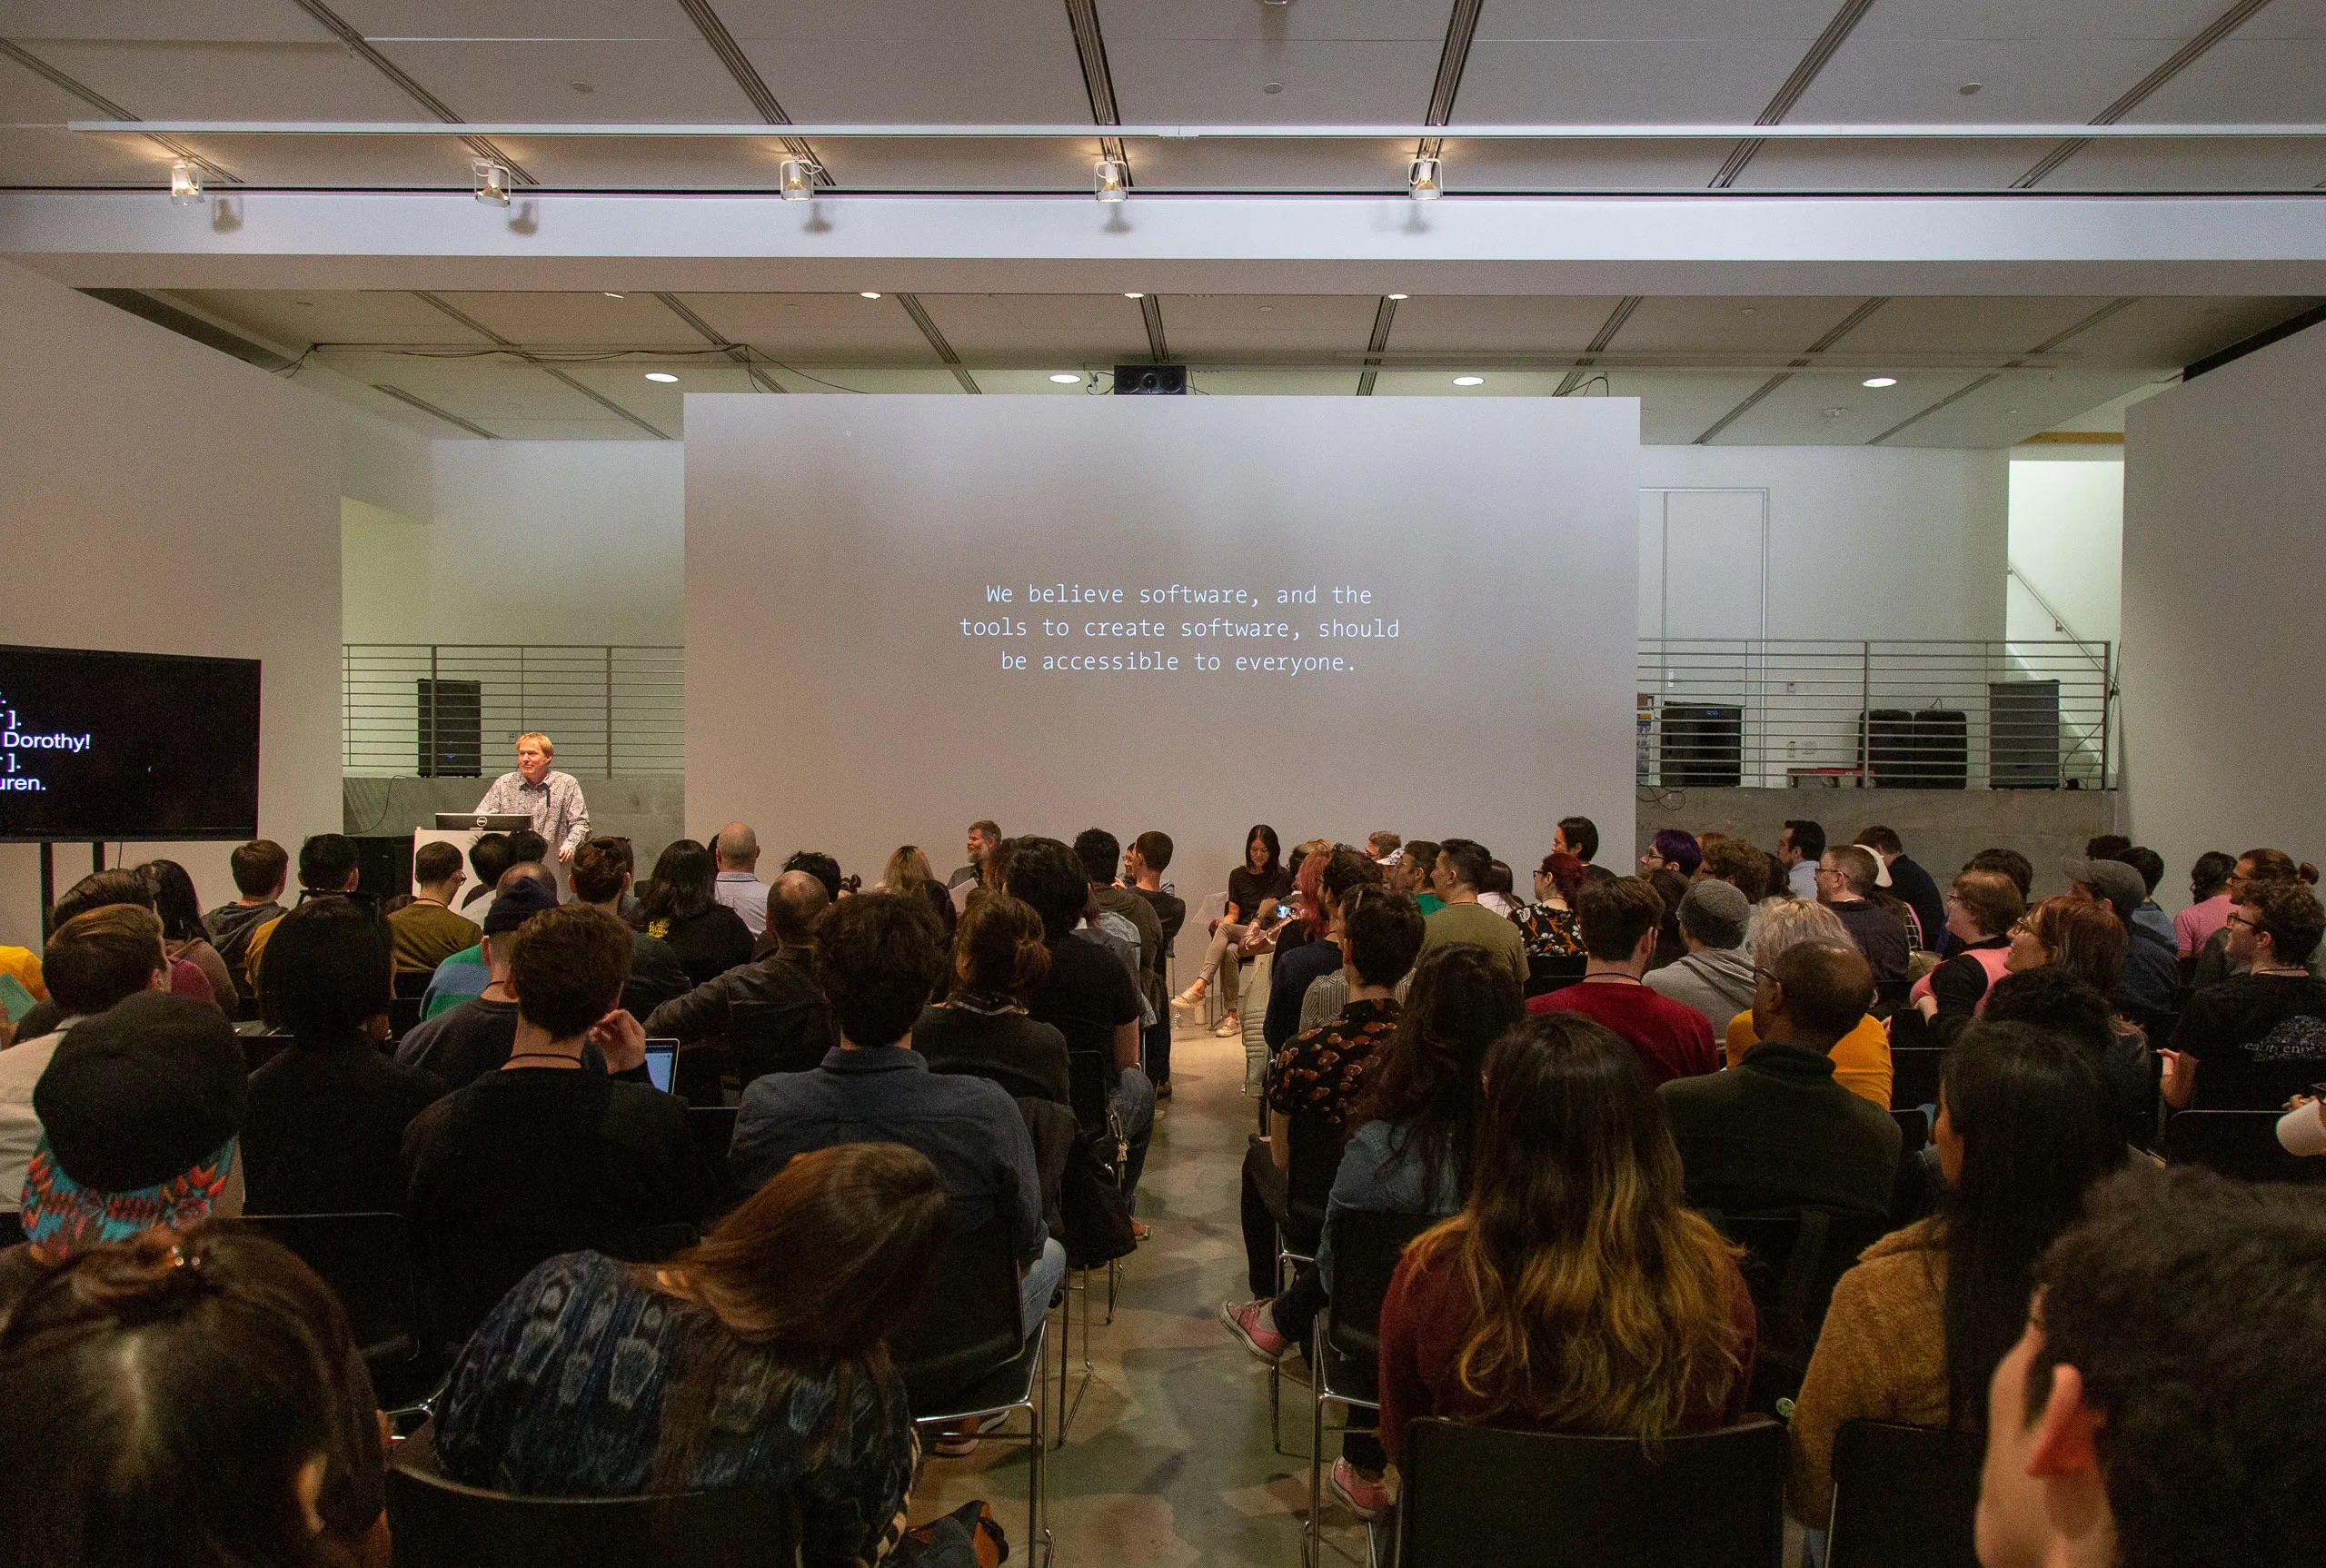
\includegraphics[width=1\textwidth]{images/pcd_la_2019.jpeg}
    \caption[Ben Fry at PCD 2018]{Ben Fry with conference attendees. Source: \citefield{guptaBenFryConference2018}{author}, Medium, \citeyear{guptaBenFryConference2018}.}
  \end{figure}
  
\subsection{Values of the Processing Project}

The success of the Processing language is evidenced by its proliferation into various flavors such as Processing for Python, Android, and p5.js, each adaptation carrying the core philosophy into new contexts and platforms. This diversification attests to the robustness and adaptability of the language, reflecting its foundational values of accessibility, diversity, and inclusivity in the realm of creative coding.

These guiding principles originate from "Processing: A Programming Handbook for Visual Designers and Artists,"\parencite{reasProcessingProgrammingHandbook2007a} which lays out the philosophical and operational framework of the Processing project. The handbook serves as a manifesto of sorts, detailing how Processing is not just a programming language but a pedagogical tool designed to bridge the gap between code and visual art. It emphasizes the unique qualities of software as a medium, advocating for a broadening understanding of programming languages as varied materials suited for different creative expressions.

The integration of sketching into the development process via Processing reflects a deliberate choice to align programming practices with those of traditional arts. This design decision underscores a commitment to making programming an intuitive and immediate experience, akin to the fluidity and exploratory nature of sketching in artistic disciplines.

By actively seeking to dismantle the barriers that have traditionally made programming an esoteric and often inaccessible field, Processing has opened its doors to a wider audience. It champions the idea that programming should be within reach of anyone with an interest in visual and spatial reasoning, not just those with a technical pedigree.

\subsection{Evaluating Design Implications in Processing}

The inception of Processing has significantly democratized the field of creative coding, with its workshop-centric educational approach enabling rapid assimilation by novices. This educational framework, spanning brief afternoon sessions to extensive week-long courses, has been pivotal in achieving the project's intent to simplify the initial learning curve for beginners. Nonetheless, the dynamic nature of the Processing API, particularly its initial shortcomings in 3D graphics, has posed challenges for more seasoned practitioners. Users with advanced aspirations, such as Karsten Schmidt, have encountered performance limitations for complex tasks, suggesting an inadvertent threshold that users may find difficult to transcend.

A latent hurdle also arises from the obscured transition between Processing's environment and the underlying Java architecture. This obscurity, as Schmidt indicates, may place constraints on learners who aim to advance, effectively curtailing their developmental trajectory. This is evidenced by users like Ariel Malka, who, finding Processing restrictive, ventured into the development of distinct projects such as Chronotext. This departure from Processing highlights its dual role as a catalyst for beginners and a potential impediment for those seeking deeper technical exploration.

Ben Fry, in our dialogue, reflected on the unanticipated loyalty of users to Processing, noting that even as projects expand in complexity, a significant number of users remain within the tool's confines, managing expansive codebases within its singular file structure. This observation raises intriguing questions about user attachment and the malleability of the tool in accommodating growing project demands.

The design choices in Processing inherently favor certain aesthetic expressions, which in turn promotes a normative creative ethos. This normativity impacts not merely the practical capabilities of the users—the 'power-to'—but also influences their cognitive and artistic inclinations—the 'power-over'. Li poignantly describes this phenomenon: "The normative ground established by a tool not only affects how users can practically accomplish things (power-to), but also structures how they think and react. This represents a trade-off by granting tool designers power-over creative practitioners. Creative practice is an opportunity to trouble power dynamics by proposing a new normative ground through making art" \parencite[65]{liRethinkingPowerDynamics2023}. It is within the creative act that these power dynamics can be critically engaged with and reimagined, challenging the normative ground laid by technological tools and opening up new avenues for artistic expression.

\begin{figure}
    \centering
    \includegraphics[max width=\textwidth]{images/normative.png}
    \caption{A representation from openprocessing.org, showcasing the prevalent aesthetic trends influenced by Processing's design framework.}
    \label{fig:normative}
\end{figure}
